% Course: 77972 -- Physical Models of Biological Systems
% Academic year: 2026--2027 | Semester: A
% Lecture number: 3 | Document chapter: 3
% Lecture date: 2026-11-03
% Title: Discrete Distributions and the Luria--Delbr{\"u}ck Fluctuation Test
% Lecturer: Dr. Amir Erez
% Notes prepared by: Eran Rehani
% Source: Transcriptions/77972 2026-11-03 שעור א [9c67909c-e195-4f20-8755-b4ee006ad172]_hosted.md
% Hosted timeline, approximate: Bayesian inference and screening 00:01--00:25;
% covariance and correlation 00:26--01:07; binomial 01:08--01:17;
% fluorescence calibration 01:18--01:35; Poisson limit 01:36--01:44;
% Luria--Delbr{\"u}ck experiment and model 01:45--02:13; generating function and MLE 02:14--02:38.
% Supporting references: models-notes-2026.pdf, chapter 3 (discrete distributions, mutation);
% Philip Nelson, Physical Models of Living Systems, chapter on randomness and mutation.
% Revision date: 2026-11-05 (diagram, terminology, references and provenance).
% Revision date: 2026-11-12 (reviewed against the Panopto recording; qualified jackpot interpretation).
% Additional transcript: Transcriptions/77972 2026-11-03 שעור א [9c67909c-e195-4f20-8755-b4ee006ad172]_panopto.md
% Hosted and caption timestamps use different timelines; do not interchange them.
% Revision date: 2026-11-12 (checked supplied Panopto transcript and clarified model comparison).
\chapter{Discrete Distributions and the Luria--Delbr{\"u}ck Fluctuation Test}\label{chap:lecture03}
\noindent\textbf{Lecture 3 \enspace|\enspace 3 November 2026}

This lecture begins with Bayesian inference and medical screening, then moves from correlation (Pearson versus Spearman, and why summary statistics can mislead) to discrete counting models: the binomial distribution, its Poisson limit, and the Luria--Delbr{\"u}ck fluctuation test of 1943. The central biological question is whether mutations arise randomly before selection (Darwin) or in response to a challenge (Lamarck). The resolution uses a probability model in which early mutations are exponentially amplified (the ``jackpot'' effect), which can produce a variance far larger than the mean for many generations. This is incompatible with the specified homogeneous Poisson alternative, but does not by itself exclude every induced-mutation model.

\begin{itemize}[nosep]
\item Apply Bayes' theorem to a rare-event screening problem; define covariance, Pearson and rank correlation; explain stationarity and correlation time.
\item \textbf{Revision goals:} derive the binomial PMF and its mean/variance; take the $M\to\infty$, $p\to0$ limit to obtain the Poisson distribution; explain the Rosenfeld $\alpha$-measurement trick via binomial partitioning at cell division; reconstruct the Luria--Delbr{\"u}ck jackpot amplification and its probability generating function; carry out the maximum-likelihood estimate of the mutation rate from zero-mutant cultures; interpret the Fano factor (variance/mean) as a diagnostic of non-Poissonian mutation.
\end{itemize}

% Hosted transcript 00:01--00:25: Bayesian inference and screening.
\section{Bayesian inference: from evidence to hypotheses}\label{sec:lecture03-bayes}
Biological measurements rarely determine a mechanism uniquely. Let $H_j$ be mutually exclusive, exhaustive hypotheses and $E$ an observation. The prior $P(H_j)$ describes uncertainty before the measurement; the likelihood $P(E\mid H_j)$ describes the measurement under a hypothesis. Their roles differ from the posterior probability of the hypothesis after observing the data.
\begin{definition}{Bayesian update}{lecture03-bayes}
For $P(E)>0$, the product rule gives
\begin{equation}\label{eq:lecture03-bayes}
P(H_j\mid E)=\frac{P(E\mid H_j)P(H_j)}{P(E)},\qquad
P(E)=\sum_kP(E\mid H_k)P(H_k).
\end{equation}
The evidence normalizes the posterior. Posterior odds equal prior odds multiplied by the likelihood ratio; the common evidence cancels.
\end{definition}
A likelihood is a function of the hypothesis with the observations fixed; it need not sum or integrate to one over hypotheses. Maximizing it does not produce a posterior distribution. For continuous parameters, a uniform prior in one coordinate need not be uniform after a nonlinear change of coordinate, because probability densities transform with a Jacobian. A prior probability of zero cannot be revived by an ordinary Bayesian update.
\begin{example}{A rare condition and an accurate test}{lecture03-screening}
This is the lecture's hypothetical probability example, not a current clinical estimate. Let $D$ denote disease and $+$ a positive test. Prevalence is $P(D)=0.009$, sensitivity is $P(+\mid D)=0.97$, and specificity is $P(-\mid D^c)=0.97$. Thus
\begin{align}
P(+)&=0.97(0.009)+0.03(0.991)=0.03846,\label{eq:lecture03-positive}\\
P(D\mid +)&=\frac{0.97(0.009)}{0.03846}\approx0.227.\label{eq:lecture03-screening}
\end{align}
A positive result raises the probability from $0.9\%$ to about $23\%$, but false positives among the much larger healthy population still outnumber true positives. Sensitivity is not the probability of disease given a positive test. Repeated results can be multiplied only when their conditional independence given disease status is justified; persistent cross-reactivity or shared handling errors can correlate them.
\end{example}

\section{Correlation: definitions, limits and remedies}\label{sec:lecture03-correlation}
% Hosted transcript 00:26--00:41: covariance and temporal/spatial correlation.
Two proteins can vary together across cells even when their absolute expression levels differ. For random variables $L,M$ with finite second moments, define
\begin{align}
\operatorname{Cov}(L,M)&=\ee[(L-\ee[L])(M-\ee[M])]
=\ee[LM]-\ee[L]\ee[M],\label{eq:lecture03-covariance}\\
\rho_{LM}&=\frac{\operatorname{Cov}(L,M)}{\sqrt{\operatorname{Var}(L)\operatorname{Var}(M)}}.\label{eq:lecture03-pearson}
\end{align}
Covariance has the product of the variables' units, and $\operatorname{Cov}(L,L)=\operatorname{Var}(L)$. Pearson's coefficient is dimensionless and requires both variances to be positive. Cauchy--Schwarz applied to the centered variables gives $|\rho_{LM}|\leq1$. Equality corresponds to an exact affine relation almost surely; independence implies zero covariance, while the converse generally fails. Specify the averaging ensemble: variation of two genes across cells and variation of two cells across genes answer different questions.

\subsection{Autocorrelation measures memory}\label{subsec:lecture03-autocorrelation}
For a stationary process $X(t)$ with mean $\bar X$ and finite variance, the centered autocovariance and its normalization are
\begin{equation}\label{eq:lecture03-autocorrelation}
C(\tau)=\ee[(X(t)-\bar X)(X(t+\tau)-\bar X)],\qquad
R(\tau)=C(\tau)/C(0).
\end{equation}
Here $C(0)=\operatorname{Var}(X)>0$ and $R(0)=1$. Stationarity makes the ensemble covariance depend on lag rather than absolute time. Estimating this ensemble average by averaging along one time trace additionally requires representative sampling, usually justified by ergodicity. Trends can create apparent memory and should be modelled or removed when appropriate. Spatial lag gives an analogous correlation length.
\begin{example}{White noise and a finite memory time}{lecture03-memory}
Discrete white noise has zero covariance at nonzero lags, not at zero lag. A possible normalized memory curve is $R(\tau)=\exp(-|\tau|/\tau_c)$, where $\tau_c$ has units of time. It describes loss of correlation over $\tau_c$; exponential decay is a model, not a universal law. The lecture's short-time Brownian-velocity example illustrates how persistence can remain before collisions randomize velocity.
\end{example}

The first part of the lecture wrapped up correlation analysis. Pearson's coefficient measures linear association only; it can be exactly zero for data with a clear nonlinear relationship (a parabola), and it can be distorted by a single outlier. Spearman's rank correlation replaces values by ranks, capturing any monotonic trend at the price of discarding the absolute scale.

\begin{remark}\label{rem:lecture03-corr-caus}
\textbf{Correlation versus causation.}
Correlation alone does not establish causal direction: $a$ may affect $b$, $b$ may affect $a$, or a common cause may affect both. Causal conclusions require interventions or additional justified causal assumptions. Perturbing one variable and measuring the response is a central experimental route.
\end{remark}

\begin{remark}\label{rem:lecture03-look-at-data}
\textbf{Look at the data.}
Summary statistics (means, variances, correlation, regression line) can be identical across data sets with radically different shapes. Always inspect the data visually before trusting summary statistics; in biology, values can span orders of magnitude and a single outlier can dominate a correlation coefficient.
\end{remark}

\begin{example}{Dependence without linear correlation}{lecture03-nonlinear}
Let $L$ take $-1,0,1$ with equal probabilities, and let $M=L^2$. Then $\ee[L]=\ee[L^3]=0$, so $\operatorname{Cov}(L,M)=0$ despite $M$ being determined by $L$. Both variances are positive and Pearson correlation is zero. A monotonic transformation is a different situation: replacing observations by their ranks before computing Pearson's coefficient gives Spearman's coefficient (using average ranks for ties). Anscombe's quartet illustrates another limitation: four data sets can share basic numerical summaries while one is curved and others are dominated by outliers. Inspect the scatter plot and residuals before interpreting a coefficient.
\end{example}

\section{The binomial distribution}\label{sec:lecture03-binomial}
A Bernoulli trial is a single experiment with two outcomes: success with probability $p$, failure with probability $1-p$. Repeating the trial $M$ independent times and counting $L$ successes gives a binomial random variable.

\begin{definition}{Binomial probability mass function}{lecture03-binomial-pmf}
The probability of observing exactly $L$ successes in $M$ independent Bernoulli trials with success probability $p$ is
\begin{equation}\label{eq:lecture03-binomial-pmf}
P(L) = \binom{M}{L} p^{L} (1-p)^{M-L},\qquad L=0,1,\ldots,M .
\end{equation}
The factor $\binom{M}{L}$ counts the number of ways to choose which $L$ of the $M$ trials succeeded.
\end{definition}

The distribution is normalized: $\sum_{L=0}^{M} P(L) = (p+(1-p))^{M} = 1$ by the binomial theorem.

\begin{proposition}{Mean and variance of the binomial}{lecture03-binomial-moments}
For $L\sim\mathrm{Binomial}(M,p)$,
\begin{equation}\label{eq:lecture03-binomial-mean}
\ee[L] = M p,
\end{equation}
and, because the $M$ trials are independent,
\begin{equation}\label{eq:lecture03-binomial-var}
\mathrm{Var}(L) = M p (1-p).
\end{equation}
\end{proposition}

\begin{proof}
Write $L = \sum_{i=1}^{M} X_i$ where $X_i\in\{0,1\}$ is the indicator of success on trial $i$. Then $\ee[X_i]=p$ and $\mathrm{Var}(X_i)=p(1-p)$. Linearity of expectation gives $\ee[L]=\sum_i\ee[X_i]=Mp$. Independence gives $\mathrm{Var}(L)=\sum_i\mathrm{Var}(X_i)=Mp(1-p)$.
\end{proof}

\section{Measuring the fluorescence proportionality constant}\label{sec:lecture03-fluorescence}

A common biological measurement uses a fluorescent protein: the fluorescence intensity $Y$ is proportional to the copy number $M$ of the protein,
\begin{equation}\label{eq:lecture03-fluorescence}
Y = \alpha M .
\end{equation}
The proportionality constant $\alpha$ bundles the labeling efficiency, fluorophore quantum yield, optical collection efficiency, and detector response. It is difficult to determine from first principles, so it must be measured in situ.

Rosenfeld et al. (2005), as cited in the lecture, used cell division for internal calibration; a 2006 paper developed the fluctuation method further. A mother cell with $M_0$ fluorescent molecules divides approximately symmetrically into two daughters. Each molecule independently goes to one daughter with probability $1/2$. Thus the number $M_1$ in daughter 1 is
\begin{equation}\label{eq:lecture03-m1-binomial}
M_1 \sim \mathrm{Binomial}(M_0,\,1/2),
\end{equation}
and $M_2 = M_0 - M_1$ in daughter 2 (no new molecules are created during division).

Condition throughout on a fixed mother count $M_0$ (equivalently fixed $Y_0$ for constant positive $\alpha$). Assume negligible synthesis, loss and measurement noise during division. Define $\Delta M=M_1-M_2=2M_1-M_0$. Its conditional mean is zero but its conditional variance is nonzero:
\begin{align}\label{eq:lecture03-deltaM-var}
\mathrm{Var}(\Delta M)
&= \mathrm{Var}(2M_1 - M_0)
= 4\,\mathrm{Var}(M_1)   \\
&= 4 \cdot M_0 \cdot \tfrac12 \cdot \tfrac12
= M_0 .
\end{align}

The measured fluorescence difference is $\Delta Y = \alpha\,\Delta M$, so
\begin{equation}\label{eq:lecture03-deltaY-var}
\mathrm{Var}(\Delta Y) = \alpha^{2}\,\mathrm{Var}(\Delta M) = \alpha^{2} M_0 .
\end{equation}
Since $Y_0 = \alpha M_0$ is the mother's fluorescence,
\begin{equation}\label{eq:lecture03-sigma-deltaY}
\sigma_{\Delta Y} = \sqrt{\mathrm{Var}(\Delta Y)} = \sqrt{\alpha^{2} M_0} = \sqrt{\alpha\,Y_0} .
\end{equation}

\begin{figure}[hbt]
\centering
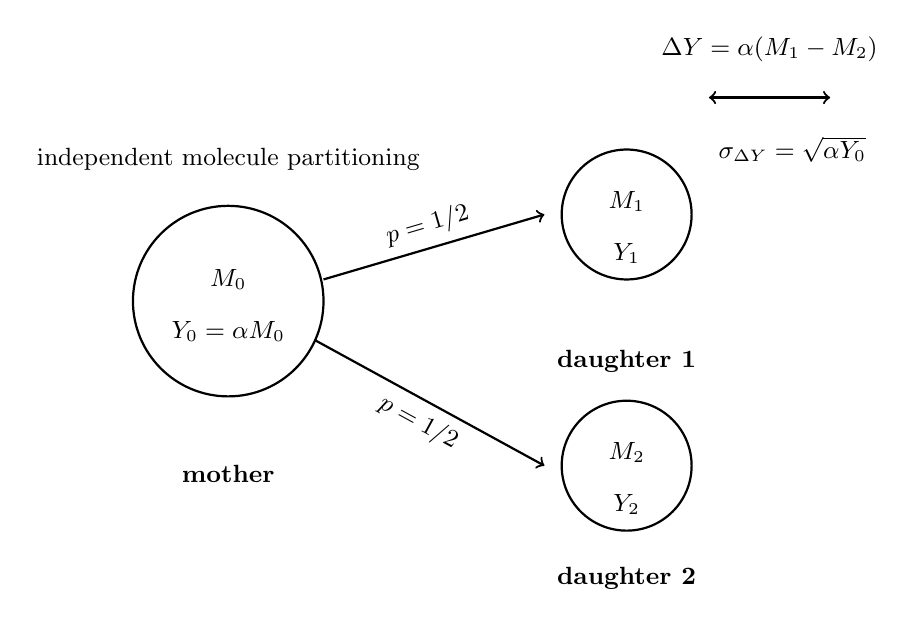
\begin{tikzpicture}[scale=1.1, every node/.style={font=\small}]
% Mother cell
\draw[thick] (0,0) circle (1.1);
\node at (0,0.25) {$M_0$};
\node at (0,-0.35) {$Y_0=\alpha M_0$};
\node at (0,-2.0) {\textbf{mother}};
% Division branches and independent partition probabilities
\draw[->,thick] (1.1,0.25) -- (3.65,1.0)
  node[midway,above,sloped] {$p=1/2$};
\draw[->,thick] (1.0,-0.45) -- (3.65,-1.9)
  node[midway,below,sloped] {$p=1/2$};
% Daughter 1
\draw[thick] (4.6,1.0) circle (0.75);
\node at (4.6,1.15) {$M_1$};
\node at (4.6,0.55) {$Y_1$};
\node at (4.6,-0.7) {\textbf{daughter 1}};
% Daughter 2
\draw[thick] (4.6,-1.9) circle (0.75);
\node at (4.6,-1.75) {$M_2$};
\node at (4.6,-2.35) {$Y_2$};
\node at (4.6,-3.2) {\textbf{daughter 2}};
% Partitioning assumption
\node[anchor=south] at (0,1.4) {independent molecule partitioning};
% Delta Y
\draw[<->,thick] (5.55,2.35) -- (6.95,2.35);
\node[anchor=south] at (6.25,2.65) {$\Delta Y=\alpha(M_1-M_2)$};
\node[anchor=west] at (5.55,1.75) {$\sigma_{\Delta Y}=\sqrt{\alpha Y_0}$};
\end{tikzpicture}
\caption{Rosenfeld calibration: symmetric partitioning of $M_0$ fluorescent molecules at cell division. The daughter-to-daughter fluorescence difference $\Delta Y$ has standard deviation $\sqrt{\alpha Y_0}$, so plotting $\sigma_{\Delta Y}$ versus $\sqrt{Y_0}$ across many mothers yields a straight line of slope $\sqrt{\alpha}$, measuring $\alpha$ in the same experiment that uses it.}
\label{fig:lecture03-rosenfeld}
\end{figure}

\begin{example}{Rosenfeld experiment}{lecture03-rosenfeld}
Measure $Y_0$ and $\Delta Y$ for many dividing bacteria. Estimate the conditional variance within narrow mother-fluorescence bins, or fit a conditional statistical model; a single daughter pair cannot supply a standard deviation. The ideal prediction for $\sigma_{\Delta Y}$ versus $\sqrt{Y_0}$ is a line of slope $\sqrt\alpha$. Measurement error, unequal partitioning, bleaching or instrument drift can cause departures and must be modelled. Once a stable conversion is inferred, $M=Y/\alpha$ converts intensity into molecule count. Calibration within the experiment reduces reliance on a separate standard but does not eliminate all systematic error.
\end{example}

\section{The Poisson limit}\label{sec:lecture03-poisson}

Take the binomial limit $M\to\infty$ with the success probability $p\to0$ such that the mean stays fixed:
\begin{equation}\label{eq:lecture03-lambda-def}
\lambda = M p \quad\text{held constant}.
\end{equation}
This is the regime of many rare independent events.

\begin{proposition}{Poisson limit of the binomial}{lecture03-poisson-limit}
As $M\to\infty$ and $p=\lambda/M\to0$,
\begin{equation}\label{eq:lecture03-poisson-pmf}
P(L) = \binom{M}{L}\left(\frac{\lambda}{M}\right)^{L}
\left(1-\frac{\lambda}{M}\right)^{M-L}
\;\longrightarrow\;
e^{-\lambda}\frac{\lambda^{L}}{L!}.
\end{equation}
The limiting distribution is Poisson with parameter $\lambda$, and
\begin{equation}\label{eq:lecture03-poisson-moments}
\ee[L]=\lambda,\qquad \mathrm{Var}(L)=\lambda.
\end{equation}
\end{proposition}

\begin{proof}
Write out the binomial PMF and separate the factors:
\begin{align}
P(L)
&= \frac{M!}{L!(M-L)!}\,
\frac{\lambda^{L}}{M^{L}}\,
\left(1-\frac{\lambda}{M}\right)^{M}
\left(1-\frac{\lambda}{M}\right)^{-L} .
\end{align}
For $M\gg L$,
\begin{equation}\label{eq:lecture03-falling-factorial}
\frac{M!}{(M-L)!\,M^{L}}
= \frac{M(M-1)\cdots(M-L+1)}{M^{L}}
\;\longrightarrow\; 1 ,
\end{equation}
since each of the $L$ factors in the numerator is $M$ up to lower-order terms. Also,
\begin{equation}\label{eq:lecture03-exp-limit}
\left(1-\frac{\lambda}{M}\right)^{M}
\;\longrightarrow\; e^{-\lambda},
\qquad
\left(1-\frac{\lambda}{M}\right)^{-L}
\;\longrightarrow\; 1 .
\end{equation}
Substituting gives $P(L)\to e^{-\lambda}\lambda^{L}/L!$. Normalization follows from $\sum_{L=0}^{\infty}e^{-\lambda}\lambda^{L}/L! = e^{-\lambda}e^{\lambda}=1$.
\end{proof}

The defining feature of the Poisson distribution is \emph{mean equals variance}. The Luria--Delbr{\"u}ck data violate it dramatically.

\section{The Luria--Delbr{\"u}ck experiment (1943)}\label{sec:lecture03-ld}

Luria and Delbr{\"u}ck (1943) grew bacteria from a single founder to a large population, then challenged the culture with a bacteriophage (virus that infects bacteria). Most bacteria were killed and the culture turned clear, but a few resistant colonies reappeared. The question: did the phage \emph{induce} resistance (Lamarck: mutation as a response to the challenge), or were resistant mutants already present \emph{before} exposure (Darwin: random mutation followed by selection)?

\begin{figure}[hbt]
\centering
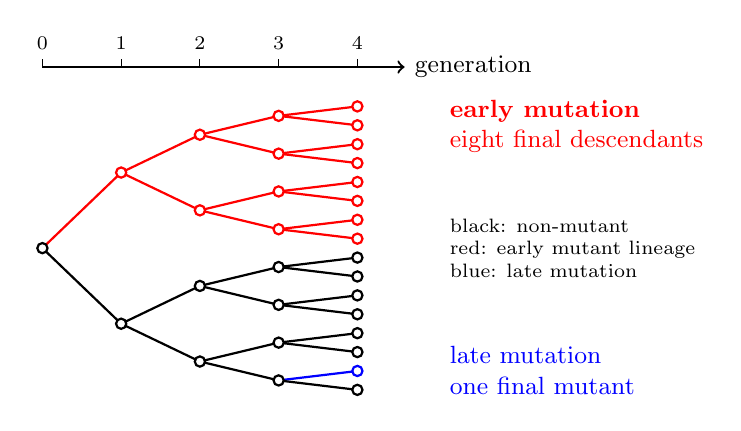
\begin{tikzpicture}[every node/.style={font=\small}]
\draw[->,thick] (0,2.3) -- (4.6,2.3) node[right] {generation};
\foreach \g in {0,...,4} {
  \draw (\g,2.3) -- (\g,2.4) node[above] {\scriptsize\g};
}
% Draw each lineage once; color the edge on which the mutation first appears.
\foreach \g in {1,...,4} {
  \pgfmathtruncatemacro{\last}{2^\g-1}
  \pgfmathtruncatemacro{\half}{2^(\g-1)}
  \foreach \k in {0,...,\last} {
    \pgfmathsetmacro{\y}{1.92-(\k+0.5)*3.84/(2^\g)}
    \pgfmathsetmacro{\yp}{1.92-(floor(\k/2)+0.5)*3.84/(2^(\g-1))}
    \def\lineagecolor{black}
    \ifnum\k<\half\def\lineagecolor{red}\fi
    \ifnum\g=4\ifnum\k=14\def\lineagecolor{blue}\fi\fi
    \draw[thick,\lineagecolor] (\g-1,\yp) -- (\g,\y);
  }
}
% Opaque nodes keep branch lines out of the cell symbols.
\foreach \g in {0,...,4} {
  \pgfmathtruncatemacro{\last}{2^\g-1}
  \pgfmathtruncatemacro{\half}{2^(\g-1)}
  \foreach \k in {0,...,\last} {
    \pgfmathsetmacro{\y}{1.92-(\k+0.5)*3.84/(2^\g)}
    \def\lineagecolor{black}
    \ifnum\g>0\ifnum\k<\half\def\lineagecolor{red}\fi\fi
    \ifnum\g=4\ifnum\k=14\def\lineagecolor{blue}\fi\fi
    \draw[thick,draw=\lineagecolor,fill=white] (\g,\y) circle (0.065);
  }
}
\node[anchor=west,align=left,text=red] at (5.05,1.55) {\textbf{early mutation}\\eight final descendants};
\node[anchor=west,align=left,font=\scriptsize] at (5.05,0) {black: non-mutant\\red: early mutant lineage\\blue: late mutation};
\node[anchor=west,align=left,text=blue] at (5.05,-1.55) {late mutation\\one final mutant};
\end{tikzpicture}
\caption{Jackpot amplification in the Luria--Delbr{\"u}ck model. A mutation occurring early (red) is present in the founder of a large subpopulation and yields many resistant descendants by the final generation (a ``jackpot'' culture). A mutation occurring late (blue) yields few descendants. Cultures are therefore highly variable: most have zero or a few mutants, rare cultures have very many.}
\label{fig:lecture03-jackpot}
\end{figure}

The experimental logic:
\begin{enumerate}[nosep]
\item Start with one bacterium; let it grow for $g$ generations to a population $N = n_0\,2^{g}$ (with $n_0=1$ founder).
\item Expose to phage. Only pre-existing resistant mutants survive.
\item Plate dilutions on selective medium and count colony-forming units (CFU): each visible colony descends from one bacterium.
\item Repeat many independent cultures and record how many resistant colonies each culture produced.
\end{enumerate}

Two competing hypotheses:
\begin{definition}{Lamarckian (induced) mutation}{lecture03-lamarck}
The challenge (phage) elicits a defensive mutation in response; resistance frequency should be similar across cultures and mutations arise only after exposure.
\end{definition}
\begin{definition}{Darwinian (spontaneous) mutation}{lecture03-darwin}
Mutations arise randomly and independently of the phage, during growth before exposure. The phage merely selects pre-existing mutants. Resistance frequency varies strongly between cultures because early mutations are amplified exponentially.
\end{definition}

The lecturer noted the historical resonance: in 1943 the structure of DNA was unknown (described by the double-helix model 10 years later), so the question could not be settled by sequencing. It had to be settled indirectly, statistically, using the same logic as the HIV resistance discussion in Lecture 1, where drug resistance mutations pre-exist rather than being induced by the drug.

\section{Jackpot amplification: the mathematics}\label{sec:lecture03-jackpot-math}

Assume synchronous, perfectly exponential growth: generation $n$ contains $n_0\,2^{n}$ bacteria. In each generation, every bacterium mutates to resistance with a small probability $\mu$, independently. The expected number of \emph{new mutation events} in generation $n$ is
\begin{equation}\label{eq:lecture03-lambda-n}
\lambda_n = \mu\,n_0\,2^{n},
\end{equation}
We approximate the number $m_n$ of new mutation events in generation $n$ by independent Poisson variables:
\begin{equation}\label{eq:lecture03-mn-poisson}
m_n \sim \mathrm{Poisson}(\lambda_n).
\end{equation}
This is a rare-mutation approximation to finite binomial opportunities, not an exact finite-population process. As discussed in the lecture, divisions are synchronous, resistance is inherited without back mutation, and repeat events in already-mutant lineages are neglected. Mutant and non-mutant lineages grow equally fast before selection. Neglecting depletion is appropriate when the mutant fraction is small (in particular, $g\mu\ll1$ for its mean). The approximation can assign counts above the final population and should not be used to describe saturation. Here $\mu$ refers to mutation opportunities assigned to cells in generation $n$; a per-division definition must be converted consistently.

A mutation that occurs in generation $n$ is inherited by all descendants. From generation $n$ to the final generation $g$ there are $g-n$ further doublings, so the amplification factor is
\begin{equation}\label{eq:lecture03-amplification}
a_n = 2^{g-n}.
\end{equation}
The number of resistant bacteria in the final generation descended from mutations that arose in generation $n$ is therefore
\begin{equation}\label{eq:lecture03-yn-def}
y_n = a_n\,m_n = 2^{g-n}\,m_n .
\end{equation}

\begin{proposition}{Equal contribution of every generation}{lecture03-equal-contribution}
The expected number of final-generation resistant bacteria attributable to mutations arising in generation $n$ is
\begin{equation}\label{eq:lecture03-equal-contribution}
\ee[y_n] = 2^{g-n}\,\lambda_n
= 2^{g-n}\,\mu\,n_0\,2^{n}
= \mu\,n_0\,2^{g}.
\end{equation}
This is independent of $n$: every generation contributes the same expected number $\mu N$ of final mutants, where $N=n_0\,2^{g}$ is the final population size.
\end{proposition}

This is the mathematical essence of the jackpot: an early mutation is rare (few cells can mutate) but is amplified into many descendants; a late mutation is likely (many cells can mutate) but is amplified into few descendants. The two effects cancel in expectation.

The total number of resistant bacteria in the final generation is
\begin{equation}\label{eq:lecture03-s-def}
s = \sum_{n=1}^{g} y_n .
\end{equation}
Its mean is
\begin{equation}\label{eq:lecture03-s-mean}
\ee[s] = \sum_{n=1}^{g} \mu N = g\,\mu\,N .
\end{equation}
At fixed $N$, the mean grows linearly with the number of generations $g$; the variance distinguishes this model from a Poisson distribution with the same mean.

\section{Probability generating functions}\label{sec:lecture03-mgf}

To handle the sum of amplified Poisson variables, the lecturer introduced the probability generating function, the discrete analogue of the Laplace transform.

\begin{definition}{Probability generating function}{lecture03-pgf}
For a discrete non-negative random variable $X$ with PMF $p(x)=\Pr(X=x)$, define
\begin{equation}\label{eq:lecture03-pgf-def}
G_X(z) = \ee[z^{X}] = \sum_{x=0}^{\infty} p(x)\,z^{x}.
\end{equation}
\end{definition}

The PGF converges for $|z|\leq1$. The moment-generating function is $M_X(t)=G_X(\ee^t)$ where finite; the two definitions use different arguments. Derivatives below are evaluated from inside the convergence domain at $z=1$ and yield finite identities when the relevant moments exist. Key properties:
\begin{enumerate}[nosep]
\item Normalization: $G_X(1) = \sum_x p(x) = 1$.
\item First moment: $G_X'(1) = \ee[X]$.
\item Second factorial moment: $G_X''(1) = \ee[X(X-1)]$, so $\mathrm{Var}(X) = G_X''(1) + G_X'(1) - (G_X'(1))^{2}$.
\item Independence: if $X$ and $Y$ are independent, then $G_{X+Y}(z) = G_X(z)\,G_Y(z)$ (generating function of a sum is the product).
\end{enumerate}

\begin{proof}
Differentiating the series twice:
\begin{align}
G_X'(z) &= \sum_{x} p(x)\,x\,z^{x-1},
&
G_X''(z) &= \sum_{x} p(x)\,x(x-1)\,z^{x-2}.
\end{align}
At $z=1$: $G_X'(1)=\sum_x p(x)x=\ee[X]$ and $G_X''(1)=\sum_x p(x)x(x-1)=\ee[X(X-1)]$.
\end{proof}

\begin{proof}
\begin{align}
G_{X+Y}(z)
&= \ee[z^{X+Y}]
= \ee[z^{X}z^{Y}]
= \ee[z^{X}]\,\ee[z^{Y}]
= G_X(z)\,G_Y(z),
\end{align}
where the step $\ee[z^Xz^Y]=\ee[z^X]\ee[z^Y]$ uses independence.
\end{proof}

For a Poisson random variable $m\sim\mathrm{Poisson}(\lambda)$,
\begin{align}\label{eq:lecture03-poisson-pgf}
G_m(z)
&= \sum_{m=0}^{\infty} e^{-\lambda}\frac{\lambda^{m}}{m!}z^{m}
= e^{-\lambda}\sum_{m=0}^{\infty}\frac{(\lambda z)^{m}}{m!}
= e^{-\lambda}\,e^{\lambda z}
= e^{\lambda(z-1)} .
\end{align}

\section{Generating function of the total mutant count}\label{sec:lecture03-gs}

Apply the generating-function machinery to $s=\sum_n y_n$ with $y_n = a_n m_n$.

For one generation,
\begin{align}\label{eq:lecture03-yn-pgf}
G_{y_n}(z)
&= \ee[z^{a_n m_n}]
= G_{m_n}(z^{a_n})
= e^{\lambda_n(z^{a_n}-1)} .
\end{align}

Since mutation events in different generations are independent, the variables $y_n$ are independent, and
\begin{align}\label{eq:lecture03-gs-def}
G_s(z)
&= \prod_{n=1}^{g} G_{y_n}(z)
= \prod_{n=1}^{g} e^{\lambda_n(z^{a_n}-1)}
= \exp\!\left(\sum_{n=1}^{g}\lambda_n\,(z^{a_n}-1)\right) .
\end{align}

This is the central object: from its derivatives at $z=1$ one obtains all moments of $s$; from its value at $z=0$ one obtains the probability of zero mutants.

\subsection{Probability of zero mutants}\label{subsec:lecture03-zero-mutants}

Setting $z=0$ in \eqref{eq:lecture03-gs-def}: since $a_n>0$, $z^{a_n}\to0$,
\begin{align}\label{eq:lecture03-gs-zero}
G_s(0)
&= \exp\!\left(-\sum_{n=1}^{g}\lambda_n\right).
\end{align}
But $G_s(0) = \Pr(s=0)$ (only the $s=0$ term in the defining sum survives), so
\begin{equation}\label{eq:lecture03-p-zero}
\Pr(s=0) = \exp\!\left(-\sum_{n=1}^{g}\lambda_n\right).
\end{equation}

Now sum the $\lambda_n$:
\begin{align}\label{eq:lecture03-lambda-sum}
\sum_{n=1}^{g}\lambda_n
&= \mu\,n_0\sum_{n=1}^{g}2^{n}
= \mu\,n_0\,(2^{g+1}-2)
\;\approx\; 2\,\mu\,n_0\,2^{g}
= 2\,\mu\,N ,
\end{align}
where the last step uses $N=n_0\,2^{g}$ and drops the subleading $-2\mu n_0$ for large $g$. The lecturer denoted this sum by $\lambda_{\mathrm{big}}\approx 2\mu N$.

\begin{remark}\label{rem:lecture03-lambda-big}
\textbf{Approximation.}
The exact sum in this convention is $\lambda_{\mathrm{big}}=2\mu(N-n_0)$. Replacing it by $2\mu N$ requires $N\gg n_0$. Consistent relabelling of generation indices cannot change this physical result; changing mutation opportunities from daughter cells to cell divisions can change the conversion between rate parameters.
\end{remark}

Therefore
\begin{equation}\label{eq:lecture03-p-zero-final}
\Pr(s=0) \;\approx\; e^{-2\mu N}.
\end{equation}

\subsection{Mean and variance from derivatives}\label{sec:lecture03-s-moments}
\textbf{Supplementary derivation.} The lecture deferred the full variance calculation to the next session. The following completes it within the independent-Poisson model stated above.

From $G_s(z)$:
\begin{align}
\ee[s] &= G_s'(1)
= \left.\frac{d}{dz}\exp\!\left(\sum_n\lambda_n(z^{a_n}-1)\right)\right|_{z=1} \\
&= \exp(0)\cdot\sum_n\lambda_n a_n
= \sum_n \lambda_n 2^{g-n}
= \sum_n \mu n_0 2^{g}
= g\,\mu\,N,
\end{align}
matching \eqref{eq:lecture03-s-mean}.

For the variance, use $G_s''(1)=\ee[s(s-1)]$:
\begin{align}
G_s''(1)
&= \left[\left(\sum_n\lambda_n a_n z^{a_n-1}\right)^{2}
+ \sum_n\lambda_n a_n(a_n-1)z^{a_n-2}\right]_{z=1}
\cdot e^{0} \\
&= \left(\sum_n\lambda_n a_n\right)^{2}
+ \sum_n\lambda_n a_n(a_n-1).
\end{align}
The first term is $(\ee[s])^2$. The second:
\begin{align}
\sum_n\lambda_n a_n(a_n-1)
&= \sum_n (\mu n_0 2^{n})\,2^{g-n}(2^{g-n}-1) \\
&= \mu n_0 2^{g}\sum_n(2^{g-n}-1)
= \mu N \sum_{k=0}^{g-1}(2^{k}-1) \\
&= \mu N \bigl((2^{g}-1) - g\bigr)
\;\approx\; \mu N\,2^{g}
= \mu N^{2}/n_0 .
\end{align}
Hence
\begin{equation}\label{eq:lecture03-s-var}
\mathrm{Var}(s) = G_s''(1) + \ee[s] - (\ee[s])^{2}
=\mu N(2^g-1)\approx\mu N^{2}/n_0.
\end{equation}

For $\mu>0$ and $g\geq1$, the Fano factor is therefore
\begin{equation}\label{eq:lecture03-pano}
\text{Fano factor} = \frac{\mathrm{Var}(s)}{\ee[s]}
=\frac{2^g-1}{g}\approx\frac{N}{g\,n_0}.
\end{equation}

For a Poisson distribution the Fano factor is exactly 1. For many generations it can be enormous: the variance is dominated by rare jackpot cultures with very large $s$. This supports pre-selection amplification against the homogeneous independent induced-mutation alternative.

\begin{remark}\label{rem:lecture03-variance-large}
\textbf{Why the variance is so large.}
Early events yield large clones and strongly increase the variance. For fixed $n_0$ and small $\mu$, the model variance grows approximately as $\mu N^2/n_0$, while a Poisson variable with the same mean has variance $g\mu N=\mu N\log_2(N/n_0)$. Whether most cultures have zero or few mutants depends on the parameters. A large Fano factor rejects the specified homogeneous independent induced-mutation model; heterogeneous or correlated alternatives require separate assessment.
\end{remark}

\section{Maximum-likelihood estimate of the mutation rate}\label{sec:lecture03-mle}

Repeat the experiment in $c\geq1$ independent cultures with common $n_0,g,\mu$ and final population $N$. Let $c_0$ be the number of cultures with zero resistant mutants ($s=0$), and $c-c_0$ the number with at least one mutant. Initially assume $0<c_0<c$. The probability model is
\begin{equation}\label{eq:lecture03-pzero-model}
\Pr(s=0) = e^{-\lambda_{\mathrm{big}}},
\qquad
\Pr(s>0) = 1 - e^{-\lambda_{\mathrm{big}}},
\end{equation}
where $\lambda_{\mathrm{big}}\approx 2\mu N$ is the expected number of mutation events per culture.

The likelihood of observing exactly $c_0$ zero-mutant cultures out of $c$ is binomial in $c_0$:
\begin{equation}\label{eq:lecture03-likelihood}
L(\lambda_{\mathrm{big}})
= \bigl(e^{-\lambda_{\mathrm{big}}}\bigr)^{c_0}
  \bigl(1-e^{-\lambda_{\mathrm{big}}}\bigr)^{c-c_0}.
\end{equation}
(The combinatorial prefactor $\binom{c}{c_0}$ does not depend on $\lambda_{\mathrm{big}}$ and can be dropped for maximization.)

The log-likelihood is
\begin{equation}\label{eq:lecture03-loglik}
\ell(\lambda_{\mathrm{big}})
= -c_0\,\lambda_{\mathrm{big}}
+ (c-c_0)\,\ln\!\bigl(1-e^{-\lambda_{\mathrm{big}}}\bigr).
\end{equation}

Maximize by setting the derivative to zero:
\begin{align}
\frac{d\ell}{d\lambda_{\mathrm{big}}}
&= -c_0
+ (c-c_0)\,\frac{e^{-\lambda_{\mathrm{big}}}}{1-e^{-\lambda_{\mathrm{big}}}}
= 0 .
\end{align}
Rearranging:
\begin{align}
c_0\bigl(1-e^{-\lambda_{\mathrm{big}}}\bigr)
&= (c-c_0)\,e^{-\lambda_{\mathrm{big}}} \\
c_0 - c_0 e^{-\lambda_{\mathrm{big}}}
&= c\,e^{-\lambda_{\mathrm{big}}} - c_0 e^{-\lambda_{\mathrm{big}}} \\
c_0 &= c\,e^{-\lambda_{\mathrm{big}}} .
\end{align}
Therefore
\begin{equation}\label{eq:lecture03-mle-lambda}
e^{-\hat{\lambda}_{\mathrm{big}}} = \frac{c_0}{c},
\qquad
\hat{\lambda}_{\mathrm{big}} = -\ln\!\frac{c_0}{c} = \ln\!\frac{c}{c_0}.
\end{equation}

Since $\lambda_{\mathrm{big}}\approx 2\mu N$, the maximum-likelihood estimate of the mutation rate is
\begin{equation}\label{eq:lecture03-mle-mu}
\hat{\mu}
= \frac{\hat{\lambda}_{\mathrm{big}}}{2(N-n_0)}
\approx \frac{1}{2N}\,\ln\!\frac{c}{c_0},
\qquad N = n_0\,2^{g}.
\end{equation}

\begin{example}{Numerical illustration}{lecture03-mle-numeric}
At the boundaries, $c_0=c$ gives $\hat\lambda_{\mathrm{big}}=\hat\mu=0$. If $c_0=0$, the likelihood increases toward its supremum as $\lambda_{\mathrm{big}}\to\infty$; there is no finite unconstrained maximum. This signals inadequate zero-culture information and does not justify a literal infinite biological mutation rate.
Suppose $c=20$ parallel cultures, of which $c_0=5$ show no resistant colonies, and the final population is $N=10^{9}$ bacteria per culture. Then
\begin{equation}\label{eq:lecture03-mle-numeric}
\hat{\mu} = \frac{1}{2\cdot10^{9}}\ln\!\frac{20}{5}
= \frac{\ln 4}{2\cdot10^{9}}
\approx \frac{1.386}{2\cdot10^{9}}
\approx 6.9\times10^{-10}
\end{equation}
mutations per bacterium per generation. The estimate depends only on the fraction $c_0/c$ of zero-mutant cultures and the final population size, not on the detailed distribution of mutant counts in the positive cultures.
\end{example}

\section{Why the result is not Poisson}\label{sec:lecture03-not-poisson}

If resistance mutations arose in response to the phage (Lamarck), each bacterium would face the same small challenge probability, independently, at the moment of exposure. Under this homogeneous independent alternative, the count is binomial, approximated for rare events by a Poisson distribution with mean $\mu N$ and Fano factor 1.

The actual model has mutations occurring \emph{during growth}, before exposure, with exponential amplification of early events. For many generations its Fano factor $\approx N/(g n_0)\gg1$ means that the variance greatly exceeds the mean. Early events produce a long tail of jackpot cultures, as observed by Luria and Delbr{\"u}ck. Whether most cultures have zero or few resistant colonies depends on the mutation rate and population size; rare jackpots can make replicate counts highly variable.

\section{Self-check before the exam}\label{sec:lecture03-selfcheck}

\begin{enumerate}[nosep]
\item Write the binomial PMF $\binom{M}{L}p^{L}(1-p)^{M-L}$ and state its mean $Mp$ and variance $Mp(1-p)$.
\item Take the limit $M\to\infty$, $p=\lambda/M\to0$ and show the result is $e^{-\lambda}\lambda^{L}/L!$ with mean=variance=$\lambda$.
\item Explain the Rosenfeld trick: why $M_1\sim\mathrm{Binomial}(M_0,1/2)$ leads to $\sigma_{\Delta Y}=\sqrt{\alpha Y_0}$, and how the slope of $\sigma_{\Delta Y}$ versus $\sqrt{Y_0}$ measures $\alpha$.
\item State the definition $G_X(z)=\ee[z^X]$ and prove $G_{X+Y}=G_XG_Y$ for independent $X,Y$.
\item For the Luria--Delbr{\"u}ck model, write $\lambda_n=\mu n_0 2^n$, $a_n=2^{g-n}$, $y_n=a_nm_n$, and derive $G_s(z)=\exp(\sum_n\lambda_n(z^{a_n}-1))$.
\item From $G_s(0)$, derive $\Pr(s=0)=e^{-\lambda_{\mathrm{big}}}$ with $\lambda_{\mathrm{big}}\approx2\mu N$.
\item Carry out the MLE derivation: show $\hat{\lambda}_{\mathrm{big}}=\ln(c/c_0)$ and $\hat{\mu}=\ln(c/c_0)/(2N)$.
\item Explain why the Fano factor $\mathrm{Var}(s)/\ee[s]\gg1$ supports pre-exposure mutation against the specified homogeneous, independent induced-mutation model, and why it does not exclude every possible induced model.
\end{enumerate}

\subsection*{Open questions / remarks}
\begin{itemize}[nosep]
\item The lecturer sketched the probability generating function at the end of the lecture and announced that the variance calculation (Fano factor $\gg1$) will be completed next week; the derivation above fills in that gap from his outline.
\item The factor of 2 reflects the stated mutation-opportunity convention, not a mere relabelling of generations.
\end{itemize}

\section*{Summary}
Bayes' theorem combines prior odds with the likelihood ratio, so even an accurate positive test can have a modest predictive value for a rare condition. Covariance and Pearson correlation capture linear association; rank correlation captures monotonic association, while neither establishes causation. Autocorrelation describes how dependence changes with time lag.

This lecture established three layers. First, the binomial distribution describes counts of successes in repeated independent trials, with mean $Mp$ and variance $Mp(1-p)$; in the many-rare-events limit it becomes Poisson, whose signature property is mean equal to variance. Second, cell division provides an internal calibration: binomial partitioning of fluorescent molecules at division lets one measure the fluorescence proportionality constant $\alpha$ from the slope of $\sigma_{\Delta Y}$ versus $\sqrt{Y_0}$ (Rosenfeld's trick). Third, the Luria--Delbr{\"u}ck fluctuation test models spontaneous mutation during exponential growth: early mutations are jackpots amplified by $2^{g-n}$, giving a generating function $G_s(z)=\exp(\sum_n\lambda_n(z^{2^{g-n}}-1))$, a zero-mutant probability $e^{-\lambda_{\mathrm{big}}}$, and a mutation-rate estimate $\hat{\mu}=\ln(c/c_0)/(2N)$. For many generations, the large Fano factor supports pre-existing mutation over the specified homogeneous independent induced-mutation alternative. Next week: completion of the variance/Fano-factor calculation from the probability generating function.

\subsection*{Further Reading}
\begingroup\small
Amir Erez, course notes, Chapter~3 (discrete distributions, mutation, Luria--Delbr{\"u}ck); Philip Nelson, \emph{Physical Models of Living Systems}, chapters on randomness in biology and mutation-selection.

S.~E. Luria and M. Delbr{\"u}ck, ``Mutations of Bacteria from Virus Sensitivity to Virus Resistance,'' \emph{Genetics} \textbf{28}(6), 491--511 (1943), the original fluctuation test.

N. Rosenfeld et al., ``Gene Regulation at the Single-Cell Level,'' \emph{Science} \textbf{307}, 1962--1965 (2005), \url{https://doi.org/10.1126/science.1106914}. See also ``A Fluctuation Method to Quantify In Vivo Fluorescence Data,'' \emph{Biophysical Journal} \textbf{91}, 759--766 (2006), \url{https://doi.org/10.1529/biophysj.105.073098}.

Q. Zheng, ``Update on Estimation of Mutation Rates Using Data From Fluctuation Experiments,'' \emph{Genetics} \textbf{171}, 861--864 (2005), \url{https://doi.org/10.1534/genetics.104.035774}.
\endgroup
